\documentclass[12pt, twocolumn]{article}

\usepackage{biblatex}
\bibliography{\jobname}

%\usepackage[print]{3201report}
\usepackage{3201report}
\setboolean{shortarticle}{true}


\title{GAs To Solve The Travelling Salesman Problem}
\def\journalname{GAs To Solve The Travelling Salesman Problem}
\author{Jacob House, Nabil Miri, Omar Mohamed, and Hassan El-Khatib}
\dates{Compiled~\today\hfill\break Submitted~December~10,~2018}
\institution{Memorial University of Newfoundland, Faculty of Science, Department of Computer Science} 
\course{Computer Science 3201}

\begin{abstract}
	This report investigates the {\em Travelling Salesman Problem} through 
	the use of a genetic algorithm (GA) employing the {\em inver-over} 
	crossover operator, a combination of scramble and swap mutations, 
	and a combination of $\mu + \lambda$ and replacement survival 
	selection operators.
\end{abstract}


\begin{document}
	\maketitle
	\section{Problem Specifications}
	%% BREAK LINES EVERY 80 CHARACTERS TO HELP GIT WITH MERGING
Wolfram MathWorld defines the Travelling Salesman Problem (TSP) as ``a 
problem in graph theory requiring the most efficient (\ie least total distance) 
Hamiltonian cycle a salesman can take through each of $n$ cities,'' for which
``no general method of solution is known.'' \cite{tsp_wolfram_alpha} The 
website also remarks that the problem is assigned to the class of NP-hard 
(non-deterministic polynomial time) problems.

Given three datasets, for territories Western Sahara, Uruguay, and Canada of 
size $29$, $734$, and $4,663$ cities, respectively, the objective has been 
to design a genetic algorithm from scratch in the Python programming language
to solve the TSP for each locale using some advanced technique(s).

The first advanced technique employed in the algorithm is the {\em inver-over}
hybrid crossover/mutation operator. 




	\section{The Inver-Over Operator}
	%% BREAK LINES EVERY 80 CHARACTERS TO HELP GIT WITH MERGING
The inver-over operator can be regarded as either a crossover or mutation 
operator because it takes information from other individuals in the GA's
mating pool, yet bases a single offspring off of a single primary parent, much 
the same way a mutation operator is unary, performing mutation on a single
individual \cite{p44}. Throughout this report, the inver-over operator will 
be referenced as a crossover operator as this was the inver-over 
algorithm's place in the GA developed.

\subsection{Usefulness}
As {\em inver-over} embodies aspects of both crossover and mutation 
operators, the operator  is designed to provide middle-ground to 
algorithms relying primarily on crossover for variation (as this is 
computationally expensive) and those relying on mutation for variety,
since this is often ineffective in escaping local minima%
\footnote{Local minima occur when the natural selection in the GA 
	narrows the gene pool towards a ostensibly optimal solution and 
	eliminates individuals that otherwise would evolve to become the 
	true optimal solution.} \cite{p44}.


\subsection{Representation}
A set $P$ of individuals of length $n$, each represented as a sequence
\begin{equation*}
i_k = \langle C_{c_k(0)}, C_{c_k(1)}, C_{c_k(2)}, \ldots, C_{c_k(n-1)} \rangle\text{,}
\end{equation*}
where $c_k\colon \{0, 1, \ldots, n-1\} \to \{ 1, 2, \ldots, n \}$ is a bijection 
between indices of $i_k$, $0 \leqslant k < \card(P)$, and city indices as 
provided in the data file, is used to denote the population. Let 
$M \subsetneq P$ be the mating pool containing individuals 
$i_{m(0)}, i_{m(1)},\ldots, i_{m(\card(M)-1)}$ with $m\colon 
\{0, \ldots, \card(M)-1\} \to \{0, \ldots, \card(P) -1\}$
 an injective function mapping individuals in the mating pool $M$ to 
their equal `self' in the population $P$.

Fitness of an individual $i_k$, denoted by $\fit(i_k)$ in the Algorithm~\ref{alg:inver-over}, is then determined by the formula in 
\eqref{eq:fit1}.
\begin{equation}
\fit(i_m) = \sum_{j=0}^{n-1} \left\lVert \overrightarrow{C_j \, C_{j+1}} \right\rVert, \label{eq:fit1} 
\end{equation}
where 
\begin{equation*}
\left\lVert \overrightarrow{C_j \, C_{j+1}} \right\rVert = \sqrt{(x_{C_{j+1}} - x_{C_j})^2 + (y_{C_{j+1}} - y_{C_j})^2}
\end{equation*}
is the Eucliean distance between cities $C_j$ and $C_{j+1}$.\footnote{
	Take indices $j$ modulo $n$ so when $j=n-1$, $(n-1)+1  \equiv 0 \pmod n$
	 and we compute the distance from the last city back to the first.} Hence
a lower fitness score is better.

\subsection{Algorithm}
The algorithm (Algorithm~\ref{alg:inver-over}) used mirrors that 
depicted in the article by Tao and Michalewicz \cite{p44}.

\begin{algorithm}[H]
	\caption{The inver-over operator}\label{alg:inver-over}
	\small
	\begin{algorithmic}[1]
		\Require
		\Statex{$\triangleright$ $M$ be the mating pool}
		\Statex{$\triangleright$ \parbox[t]{0.9\linewidth}{$0 \leqslant i < \card(M)$ be the index of the initial parent}}
		\Statex{$\triangleright$ $n$ be the number of cities in the tour}
		\Ensure
		\Statex{$\triangleright$ New offspring individual created}
		\Statex
		\State{\textbf{var} $child := M[i]$} \Comment{Copy the parent}
		\State{\textbf{var} $unused := \{x \in \mathbb Z \mid 0 \leqslant x < n-1\}$} 
		\State{\textbf{var} $p := \frac{1}{2}$} 
		\State{\textbf{var} $c := \rand(unused)$} \Comment{Select randomly}
		\State{$unused  := unused\,\backslash\{c\}$}
		\While{$\card(unused) > 0$}
		\If{$\rand\{x \in \mathbb R \mid 0 \leqslant x < 1\} < p$}
		\State{$c' := \rand(unused)$}
		\Else
		\State{$newPar := \rand(M)$} 
		\State{$newParC := \where(newPar = child[c])$}
		\Statex \Comment{Index $j$ in $newPar$}
		\State{$c' := newParentC + 1$}
		\EndIf
		\State{$unused := unused\,\backslash\{c'\}$}
		\If{$child[c\pm1] = child[c']$}
		\State{\textbf{break} from the \textbf{while} loop}
		\EndIf
		\State{$child[c:c'] := child[c':c]$} \Comment{Invert}
		\State{$c := c'$}
		\EndWhile
		\If{$\fit(child) \geqslant \fit(M[i])$}
		\State{\textbf{return} $child$}
		\Else 
		\State{\textbf{return} $M[i]$}
		\EndIf 
	\end{algorithmic}
\end{algorithm}

Here $M[i]$ is the primary parent from which the child is based. 
One can observe that all changes are then made to this individual, 
like a mutation, yet they involve other individuals, denoted $newPar$,
 in the mating pool.

We borrow the following example of a single iteration of the algorithm 
from Tao and Michalewicz.
\begin{enumerate}
	\item Let $child = \langle 2, 3, 9, 4, 1, 5, 8, 6, 7\rangle$ and the current
	city index $c$ is $1$ so $child[c] = 3$.
	\item \begin{enumerate}
		\item Suppose the random number generated by 
		 $\rand\{x \in \mathbb R \mid 0 \leqslant x < 1\}$
		 does not exceed $p$. Another city index $c'$ from the child is 
		 selected, say $c' = 6$ so $child[c'] = 8$. The section of $child$ 
		 after indices $c$ and $c'$ (\ie $\langle 9, 4, 1, 5, 8 \rangle$) is 
		 inverted, leaving $child = \langle 2, 3, 8, 5, 1, 4, 9, 6, 7 \rangle$.
		\item Otherwise, another individual is (randomly) selected from the
		mating pool to become the new parent. Let this be 
		$\langle 1, 6, 4, 3, 5, 7, 9, 2, 8 \rangle$. Here the city next to 
		$child[c] = 3$ is city $5$. So, the segment of $child$ to invert is 
		that which starts after city 3 and terminates after city 5 
		(\ie $\langle 9, 4, 1, 5 \rangle$). This 
		leaves $child = \langle 2, 3, 5, 1, 4, 9, 8, 6, 7\rangle$.
	\end{enumerate}
\end{enumerate}
As in Tao and Michalewicz, we remark that in either case the resulting 
string is intermediate in the sense that the above inversion operator is 
applied several times before an offspring is evaluated. After a number
of iterations, suppose $child = \langle 9, 3, 6, 8, 5, 1, 4, 2, 7\rangle$ 
and $c = 2$ so $child[c] = 6$.
\begin{enumerate}
	\setcounter{enumi}{2}
	\item \begin{enumerate}
		\item  If $\rand\{x \in \mathbb R \mid 0 \leqslant x < 1\}$ is greater
		than $p$, the city following $child[c] = 6$ is selected from a 
		randomly chosen individual in the mating pool $M$. Let this 
		city be city $8$. As $8$ follows $6$ in $child$, the algorithm 
		terminates.
		\item Otherwise, a randomly selected city is chosen. This may 
		also be $8$, in which case the algorithm also terminates. If it is 
		not $8$, the algorithm continues as described in (2).
	\end{enumerate}
\end{enumerate} 
	\section{Our Algorithm}
	%% BREAK LINES EVERY 80 CHARACTERS TO HELP GIT WITH MERGING

	\section{Optimization}
	%% BREAK LINES EVERY 80 CHARACTERS TO HELP GIT WITH MERGING

	\section{Results}
	%% BREAK LINES EVERY 80 CHARACTERS TO HELP GIT WITH MERGING
With the optimizations discussed in Section~\ref{ssec:precomputing}, 
pre-processing speeds increased dramatically from near-negligible time
to load the file to the times listed in Table~\ref{tab:precomputing}.
Note that there are only three entries per data set as pre-processing was 
done outside the |main()| function to save computation (\ie pre-processing
was done once for every 10 trials).
\begin{table}[h]
	\centering\small
	\def\arraystretch{1}
	\begin{tabular}{>{\bf}*4{c}} \hline 
		\textbf{Trial} & \textbf{Western Sahara} & \textbf{Uruguay} & \textbf{Canada} \\ \hline 
		1 & $112.342$ & $769.979$ & $31302.409$  \\
		2 & $110.887$ & $774.185$ & $30910.104$ \\
		3 & $110.485$ & $725.295$ & $30977.966$ \\ \hline 
	\end{tabular}
	\caption{Distance Pre-computation Times (ms)\label{tab:precomputing}}	
\end{table}
Execution of the GA was done with $5,000$ generations for each dataset 
with each generation taking approximately $400$, $1,200$, and $4,600$ 
milliseconds for Western Sahara, Uruguay, and Canada datasets, respectively.
For the smallest dataset, Western Sahara, $5,000$ proved to be a rather large 
number of iterations as the last generation with improved fitness hovers 
around $1,500$ (Table~\ref{tab:last-gen-tiny}). 
\begin{table}[H]
	\centering\small
	\tabcolsep=2pt
	\def\arraystretch{1}
	\begin{tabular}{*3{c}} \hline 
		\textbf{Trial} & \parbox{1.5cm}{\centering\bfseries Last\\Improve.} & \parbox{1.5cm}{\centering\bfseries Best\\Fitness} \\ \hline 
		1 & 1308 & 27620 \\
		2 & 4012 & 30664 \\
		3 & 2889 & 27768 \\
		4 & 3271 & 28513 \\
		5 & 4103 & 27768  \\
		6 & 3158 & 28202 \\
		7 & 1716 & 28202 \\
		8 & 1059 & 29154 \\
		9 & 1948 & 29098 \\
		10 & 2199 & 30048 \\
		11 & 4639 & 29177 \\
		12 & 1710 & 28039 \\
		13 & 839 & 27748 \\
		14 & 729 & 29686 \\
		15 & 597 & 29373 \\ \hline 
	\end{tabular}
	\begin{tabular}{*3{c}} \hline 
		\textbf{Trial} & \parbox{1.5cm}{\centering\bfseries Last\\Improve.} & \parbox{1.5cm}{\centering\bfseries Best\\Fitness} \\ \hline 
		16 & 1056 & 29337 \\
		17 &1407  & 27768 \\
		18 & 1686 & 28728 \\
		19 & 1078 & 28765 \\
		20 & 2371 & 28061 \\
		21 & 1534 & 28249 \\
		22 & 610 & 28735 \\
		23 & 4890 & 27620 \\
		24 & 2484 & 28249 \\
		25 & 803 & 29535 \\
		26 & 990 & 28231 \\
		27 & 1224 & 30709 \\
		28 & 810 & 30502 \\
		29 & 683 & 28222 \\
		30 & 4582 & 28755 \\ \hline 
	\end{tabular}
	\caption{Last Generation With Improvement (Western Sahara)\label{tab:last-gen-tiny}}
\end{table}
Consequently, Figure~\ref{fig:tiny-fitnesses} 
illustrates a plateau fairly early in the execution. This means that in 
some cases, similar results could be obtained much faster, with much
less computation. On the other hand, some trials have improvement 
as far as nearly $4,900$ generations into execution. Such trials sometimes
are the ones with the most optimal fitness (\eg trials $5$ and $23$
had improvement in generation $4,103$ and $4,890$, respectively 
and finished with best fitnesses of $27,768$ and $27,620$).
\begin{figure*}[h]
	\centering
	\fbox{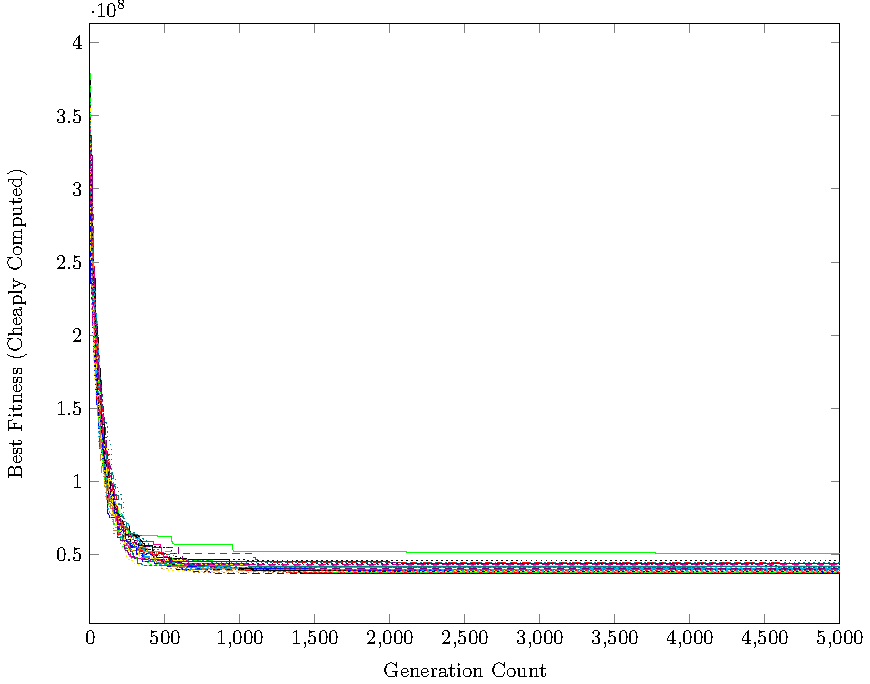
\includegraphics[width=0.65\linewidth]{include/graphs/fitness/tiny-fitnesses-lg}}
	\caption{Fitness Changes over $5,000$ Generations (Western Sahara)\label{fig:tiny-fitnesses}}
\end{figure*}
According to the University of Waterloo's Faculty of Mathematics, optimal fitness for this tour is $27,603$ \cite{sahara}. Therefore, several of the trials logged in Table~\ref{fig:tiny-fitnesses} show the algorithm's effectiveness in reaching near-optimal solutions. Given time to run more generations, optimal solutions should be achieved.

Uruguay, on the other hand, did not plateau in the same way that 
Western Sahara did (Figure~\ref{fig:med-fitnesses}).
\begin{table}[H]
	\centering\small
	\tabcolsep=2pt
	\def\arraystretch{1}
	\begin{tabular}{*3{c}} \hline 
		\textbf{Trial} & \parbox{1.5cm}{\centering\bfseries Last\\Improve.} & \parbox{1.5cm}{\centering\bfseries Best\\Fitness} \\ \hline 
		1 & 4995 & 682092 \\
		2 & 4987 & 686624 \\
		3 & 4991 & 675225 \\
		4 & 4993 & 675225 \\
		5 & 4974 & 685579  \\
		6 & 4990 & 673494 \\
		7 & 4996 & 689418 \\
		8 & 4996 & 678421 \\
		9 & 4995 & 659951 \\
		10 & 4999 & 687908 \\
		11 & 4987 & 680266 \\
		12 & 4988 & 699569 \\
		13 & 4998 & 702853 \\
		14 & 4993 & 696526 \\
		15 & 4995 & 701105 \\ \hline 
	\end{tabular}
	\begin{tabular}{*3{c}} \hline 
		\textbf{Trial} & \parbox{1.5cm}{\centering\bfseries Last\\Improve.} & \parbox{1.5cm}{\centering\bfseries Best\\Fitness} \\ \hline
		16 & 4993 & 687626 \\
		17 &4996  & 683809 \\
		18 & 4989 & 691854 \\
		19 & 4995 & 705421 \\
		20 & 4995 & 672055 \\
		21 & 4996 & 686104 \\
		22 & 4967 & 685925 \\
		23 & 4990 & 674031 \\
		24 & 4981 & 687605 \\
		25 & 4999 & 707432 \\
		26 & 4991 & 681644 \\
		27 & 4995 & 671644 \\
		28 & 4987 & 702787 \\
		29 & 4993 & 690934 \\
		30 & 4999 & 694009 \\ \hline 
	\end{tabular}
	\caption{Last Generation With Improvement (Uruguay)\label{tab:last-gen-med}}
\end{table}
\begin{figure*}[h]
	\centering
	\fbox{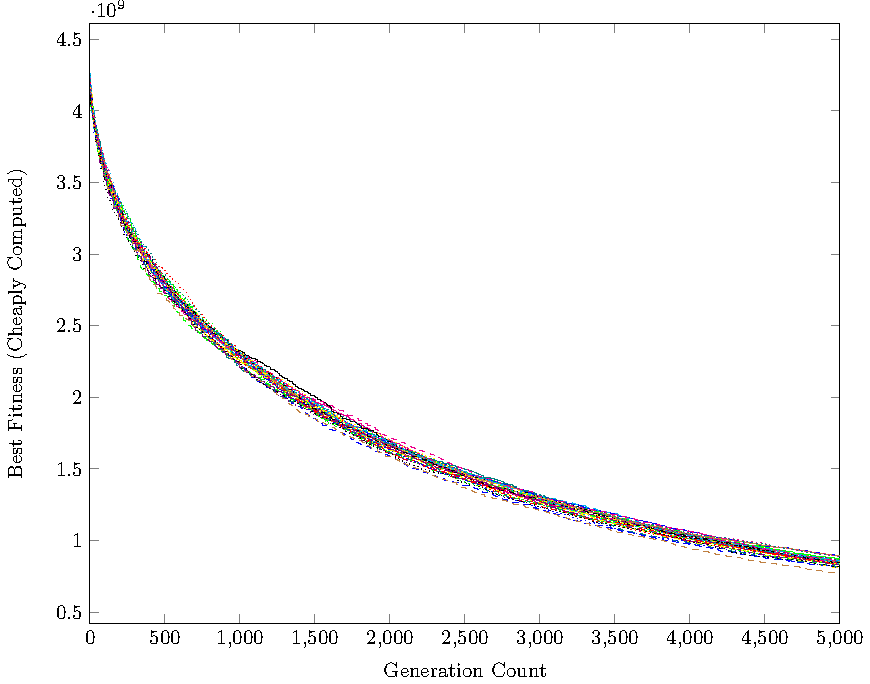
\includegraphics[width=0.65\linewidth]{include/graphs/fitness/med-fitnesses-lg}}
	\caption{Fitness Changes over $5,000$ Generations (Uruguay)\label{fig:med-fitnesses}}
\end{figure*}
This can be seen both by the way that Figure~\ref{fig:med-fitnesses}
maintains a relatively steep slope all the way to the last generation, 
as well as the high frequency of improvements above $4,980$ generations in
Table~\ref{tab:last-gen-med}.
Consequently, the algorithm, given more time to compute more generations,
should yield similar results as were demonstrated for Western Sahara.

Execution for the Canada dataset ran successfully for a number of trials,
however, due to the technique of running ten trials of the algorithm per execution,
technical errors mid-way through execution spoiled the data for all trials. 
	\section{Conclusion}
	%% BREAK LINES EVERY 80 CHARACTERS TO HELP GIT WITH MERGING
Results gathered from execution of the algorithm with the Western Sahara
dataset demonstrate the developed algorithm's efficacy in solving
the TSP. One improvement that the results from the Western Sahara
dataset indicate is a need for more effective local minima escaping 
techniques. Table~\ref{tab:last-gen-tiny} shows that in some cases
a high number of generations was required to achieve a near-optimal 
fitness, however Figure~\ref{fig:tiny-fitnesses} demonstrates a severe
plateau of best generational fitness around $500$ generations.

A more effective technique to escape local minima would reduce the 
number of generations with no improvement while still striving for 
near-optimal solutions.

While not as optimal, the results from the Uruguay dataset
do make sense and provide more useful information of where improvements
to the algorithm could be made. Extrapolation from 
Figure~\ref{fig:med-fitnesses} indicates that running more generations would likely 
result in a plateau of the best generational fitness much nearer the true
optimal solution. However, as execution for all datasets was done with
a constant population and mating pool size while the number of 
possible individuals grew at a rate of $n!$ for $n$ cities, future 
tests should be done with population and mating pool sizes that are not 
kept constant, but rather increase with the tour length. This would allow 
more variety in the population and hence could promote more diverse 
offspring, capable of escaping local minima faster and without 
reliance on severe mutation for randomness.
	\printbibliography
\end{document}